\chapter{対称性の破れ、ゴールドストーンボソン、ゲージ不変性}

光子のような粒子がどのように質量を獲得しうるのかを理解したい。それが到達点であるが、妥当な出発点ではない。ゲージ場に対する直接的な質量項は、理論を整合的にするまさにそのゲージ不変性を破壊するように見える。脱出路が見えるようになる前に、二つの考えを実用的な形で必要とする：
\begin{enumerate}
  \item 自発的対称性の破れ、特に連続対称性に対するもの；
  \item ゲージ不変性、そこでは対称性の操作が時空のある点から別の点へと変化しうる。
\end{enumerate}
どちらの考えもスローガンで置き換えることはできない。まず第一の考えを磁石から構築し、それをスカラー場の理論に翻訳し、質量のないゴールドストーンモードを発見する。次に同じ\(U(1)\)対称性を取り上げ、それを局所的にする。それによりベクトルポテンシャルと共変微分を導入せざるを得なくなる。最後になって初めて、二つの糸が並べられる。それらの実際の統合---ヒッグス現象---は次講の主題である。

\section{対称な法則と非対称な基底状態}

\subsection{二状態磁石}

小さな磁石の格子から始めよう。各スピンは上または下を向くことができ、隣り合うスピンは同じ方向を向くことによってエネルギーを下げる。三次元立方格子上では、スピンは六つの最近接隣接を持つが、正確な配位数は重要ではない。重要なのは規則
\begin{equation}
  E_{\parallel}<E_{\rm antiparallel}.
\end{equation}
である。微視的規則は、すべてのスピンを反転しても変わらない：
\begin{equation}
  \uparrow\longleftrightarrow\downarrow.
\end{equation}
それにもかかわらず、最低エネルギーの配置は個々には対称ではない。それらは
\begin{equation}
  \{\uparrow\uparrow\uparrow\cdots\},
  \qquad
  \{\downarrow\downarrow\downarrow\cdots\}.
\end{equation}
である。方程式は両方を許すが、冷たい巨視的試料は一方を選ばなければならない。

この選択は極めて敏感である。非常に遠く離れた一つのスピンを上向きに固定する。その隣接スピンはそれに従うことを好み、それらの隣接スピンは彼らに従うことを好み、情報は試料を通って伝播する。全系と比べて任意に小さな摂動が、基底状態全体の向きを選択しうる。これが\emph{自発的}対称性の破れによって意味される不安定性である。

\begin{classroomqa}
\audiencequestion{中性粒子は磁場中で自らを配向させることができるか？
\lecturetimestamp{00:05:14}}
\lecturerresponse{はい。電気的中性は磁気モーメントの不在を意味しない。中性子は中性であるが、その内部の荷電構成要素のために磁気モーメントを持つ。したがって磁場はそのスピンの向きを区別しうる。}
\end{classroomqa}

\begin{classroomqa}
\audiencequestion{系が向きを変えるなら、その変化は一度にどこでも起こるのか？複数の再配向波が共存しうるか？
\lecturetimestamp{00:05:41--00:06:38}}
\lecturerresponse{変化は伝播する。一つの領域が隣接領域を傾け、三次元のドミノ配列のように、擾乱は波として伝わる。異なる領域は独立に選択を始めうるので、一つの向きが勝つ前に複数の前線と複数のドメインが存在しうる。対称性が連続的になるとき、まさにこれらの波に戻るであろう。}
\end{classroomqa}

\subsection{明示的破れは異なる理論である}

次に試料を上向きの外部磁場中に置く。孤立したスピンはすでに上を向くときにより低いエネルギーを持つ。変換
\(\uparrow\leftrightarrow\downarrow\)
はもはやエネルギーを不変に保たない：選好が法則そのものに挿入されたのである。これが\emph{明示的}対称性の破れである。

その違いは、試料がどのように準備されたかを知らなくても試験できる。非常に大きな試料を取り、その左境界を上に固定し、右境界を下に固定する。もしバルク磁場が明示的に上を好むなら、右側の拘束は短い距離しか浸透しない。巨視的な下領域はその体積に比例するエネルギーを支払うことになるので、バルクは等しく良好な二つの相に分かれたままでいることはできない。

外部バイアスがなければ、上と下は同じバルクエネルギーを持つ。そのとき最低エネルギーの拘束状態は、上ドメイン、下ドメイン、およびそれらの間の有限の遷移層を含む。界面は幾何学的中心に位置する必要はないが、一方の相が他方を消し去ることを強制する体積圧力は存在しない。この界面は\emph{ドメイン壁}であり、この破れた離散対称性の特徴的な欠陥である。

\begin{figure}[htbp]
\centering
\begin{adjustbox}{max width=\linewidth}
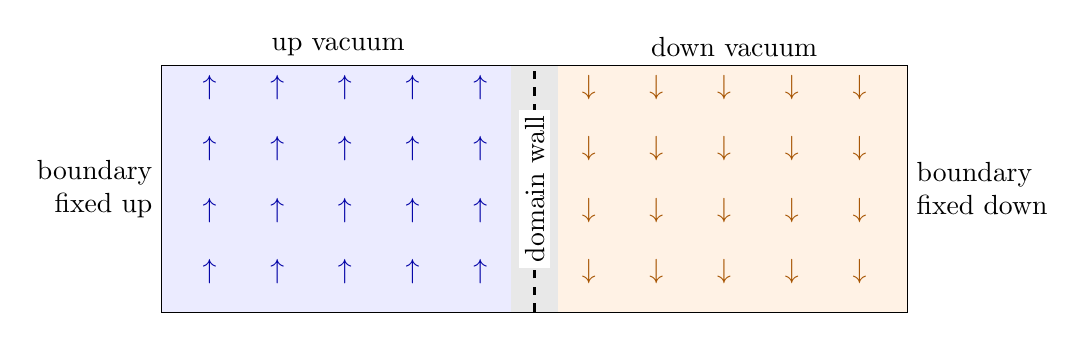
\begin{tikzpicture}[x=0.86cm,y=0.78cm]
  \draw[thick] (0,0) rectangle (11,4);
  \fill[blue!8] (0,0) rectangle (5.15,4);
  \fill[orange!10] (5.85,0) rectangle (11,4);
  \fill[gray!18] (5.15,0) rectangle (5.85,4);
  \foreach \x in {0.7,1.7,2.7,3.7,4.7}
    \foreach \y in {0.65,1.65,2.65,3.65}
      \node[blue!65!black] at (\x,\y) {$\uparrow$};
  \foreach \x in {6.3,7.3,8.3,9.3,10.3}
    \foreach \y in {0.65,1.65,2.65,3.65}
      \node[orange!65!black] at (\x,\y) {$\downarrow$};
  \draw[dashed,thick] (5.5,0) -- (5.5,4);
  \node[above] at (2.6,4) {up vacuum};
  \node[above] at (8.45,4) {down vacuum};
  \node[rotate=90,fill=white,inner sep=2pt] at (5.5,2) {domain wall};
  \node[left,align=right] at (0,2) {boundary\\fixed up};
  \node[right,align=left] at (11,2) {boundary\\fixed down};
\end{tikzpicture}
\end{adjustbox}
\caption{離散対称性の自発的破れに対する境界試験。両方のバルクの向きは同じエネルギーを持つので、壁は巨視的ドメインを分離しうる。}
\end{figure}

\begin{classroomqa}
\audiencequestion{この議論では、最近接の間の相互作用だけが必要なのだろうか。\lecturetimestamp{00:18:18}}
\lecturerresponse{いいえ。整列を好む第二近接の相互作用も、詳細は変えるが結論は変えない。より興味深い振る舞いは、異なる距離範囲が競合する場合に現れる---例えば、最近接は整列を好むが、次近接は反整列を好む場合である。これはフラストレーションとより複雑な秩序相を生むが、ここで行っている基本的な区別を変えるものではない。}
\end{classroomqa}

\begin{classroomqa}
\audiencequestion{\emph{自発的}とは、壁の内部にある大きな導関数を指すのか。\lecturetimestamp{00:19:05}}
\lecturerresponse{いいえ。それは、基礎となるエネルギーには上--下の選好がないのに、選ばれた基底状態にはそれが存在するという事実を指す。任意に小さな摂動に対する劇的な応答は、不安定性を明らかにする。勾配は、界面にどれだけのコストがかかるかを教えるにすぎない。}
\end{classroomqa}

\begin{classroomqa}
\audiencequestion{物質はすでに二つの状態の一方にあったのか、それともその状態は最初は不明だったのか。\lecturetimestamp{00:19:40}}
\lecturerresponse{それはその履歴による。高温では熱運動により、上向きスピンと下向きスピンが混ざり、平均磁化はほぼゼロになりうる。物質が冷えるにつれて、領域は異なる向きを選び、ドメイン壁が形成され、ドメインは粗大化する。偶然と微小な環境摂動が、最終的にどの真空が試料の大部分を占めるかを決める。}
\end{classroomqa}

\section{スカラー場の理論と同じ議論}

スピンを実スカラー場\(\phi(\bm{x},t)\)で置き換える。計量と規格化の規約を一度定めたら、次のように書く。
\begin{equation}
\begin{aligned}
  \mathcal L
  &=\frac12\,\partial_\mu\phi\,\partial^\mu\phi-V(\phi),
  \\
  \mathcal E
  &=\frac12\dot\phi^{\,2}+\frac12(\nabla\phi)^2+V(\phi).
\end{aligned}
  \label{eq:l07-real-scalar}
\end{equation}
\(\mathcal L\)における相対論的略記には、正の時間微分項と負の空間勾配項が含まれる。ハミルトニアンのエネルギー密度では、両方の寄与が正である。

二つの縮退した極小をもつ偶関数ポテンシャルを選ぶ。
\begin{equation}
  V(\phi)=\frac{\lambda}{4}\left(\phi^2-f^2\right)^2,
  \qquad \lambda>0.
  \label{eq:l07-double-well}
\end{equation}
ラグランジアンは\(\phi\mapsto-\phi\)の下で不変であるが、一様な真空
\begin{equation}
  \phi(\bm{x})=+f,
  \qquad\hbox{or}\qquad
  \phi(\bm{x})=-f
\end{equation}
はいずれか一方の側を選ぶ。対照的に、\(\phi=0\)に唯一の極小をもつポテンシャルは、対称な真空をもち、自発的に破れていない。

試料の一方の側で\(\phi=+f\)を、もう一方の側で\(\phi=-f\)を固定する。場はコストなしに跳ぶことはできない。なぜなら
\begin{equation}
  E_{\rm wall}
  =\int dx\left[
      \frac12\left(\frac{d\phi}{dx}\right)^2+V(\phi)-V(f)
    \right].
  \label{eq:l07-wall-energy}
\end{equation}
急激な跳びは\(d\phi/dx\)を巨大にするからである。したがって、最小エネルギーの壁は変化を有限の幅に広げ、勾配エネルギーと極小間を通るポテンシャルのコストを釣り合わせる。式~\eqref{eq:l07-double-well}のポテンシャルに対するよく知られたキンク解は
\begin{equation}
  \phi_{\rm wall}(x)
  =f\tanh\!\left[f\sqrt{\frac{\lambda}{2}}\,(x-x_0)\right],
  \label{eq:l07-kink}
\end{equation}
であり、黒板で述べられた滑らかな遷移の明示的な実現である。\editorialnote{この講義はポテンシャルの形と勾配項から議論するが、場の方程式は解かない。式
\eqref{eq:l07-kink}は、その述べられたモデルの標準的な解として含められており、議論を変えることなく定性的な壁を具体的にする。}

二重井戸をわずかに傾けると、一方の極小が低くなる。そのときラグランジアン自体が非対称になる。壁は一時的には依然として現れうるが、より高いエネルギーの真空、すなわち偽の真空が壁に圧力を及ぼす。壁は動き、好まれた相が膨張する。これは、外部磁場による明示的破れの場の理論版である。

これまでは対称性は離散的であった。素粒子物理学は\(U(1)\)、\(SU(2)\)、\(SU(3)\)のような連続群によって支配されている。連続対称性は欠陥の話を変え、新しい種類の粒子を導入する。

\section{複素場と大域的\texorpdfstring{\(U(1)\)}{U(1)}}

\subsection{内部平面における回転}

次のように置く。
\begin{equation}
  \phi=\phi_R+i\phi_I,
  \qquad
  \phi^*=\phi_R-i\phi_I,
  \qquad
  \phi^*\phi=\phi_R^2+\phi_I^2.
  \label{eq:l07-components}
\end{equation}
\(\phi_R\)軸と\(\phi_I\)軸は内部場の空間をなし、通常空間における二つの方向ではない。複素スカラーは、この内部平面における回転が明白になるようにまとめられた、単に二つの実スカラー場である。

\begin{figure}[htbp]
\centering
\includegraphics[width=0.80\textwidth]{lecture_07_figure_02.png}
\caption{内部\((\phi_R,\phi_I)\)平面における複素場。黒板には\(\phi\)と\(\phi^*\)の分解、および不変な半径\(\phi^*\phi\)が記録されている。}
\lectureframe{00:33:33}
\end{figure}

ラグランジアン
\begin{equation}
  \mathcal L
  =\partial_\mu\phi^*\,\partial^\mu\phi
   -V(\phi^*\phi).
  \label{eq:l07-complex-lagrangian}
\end{equation}
を用いる。複素場では従来の因子\(1/2\)は現れない。この単一の積がすでに両方の実成分の運動項を含んでいるからである。変換
\begin{equation}
  \phi'(x)=e^{i\theta}\phi(x),
  \qquad
  \phi^{*\prime}(x)=e^{-i\theta}\phi^*(x)
  \label{eq:l07-global-u1}
\end{equation}
はすべての場の値を同じ角度だけ回転させる。ここで\(\theta\)は空間的にも時間的にも一定である。プライムは変換された場を表し、導関数ではない。

\(\theta\)が一定であるから、
\begin{equation}
  \partial_\mu\phi'=e^{i\theta}\partial_\mu\phi,
  \qquad
  \partial_\mu\phi^{*\prime}
  =e^{-i\theta}\partial_\mu\phi^*.
\end{equation}
位相は運動項で相殺し、
\(\phi^{*\prime}\phi'=\phi^*\phi\)となる。したがって、\(\phi^*\phi\)のみに依存するすべてのポテンシャルは同じ対称性をもつ。\(\phi_R\)のみに依存する項は、内部平面における方向を選び、それを明示的に破るであろう。

\subsection{点状の極小と極小の円}

質的に異なる2つの対称なポテンシャルがある。第1のものは原点にのみ極小をもち、例えば
\begin{equation}
  V_{\rm unbroken}=m^2\phi^*\phi,
  \qquad m^2>0.
\end{equation}
である。そのグラフは回転対称な放物面である。真空\(\phi=0\)はあらゆる回転の下で固定されたままなので、対称性は破れていない。

ここで
\begin{equation}
  V_{\rm broken}
  =-a\,\phi^*\phi+b(\phi^*\phi)^2,
  \qquad a,b>0.
  \label{eq:l07-mexican-hat}
\end{equation}
を選ぶ。負の二次項は場を原点から遠ざけ、正の四次項は場が無限遠へ走るのを防ぐ。
\(r^2=\phi^*\phi\)
と書くと、最小化により
\begin{equation}
  \frac{dV}{d(r^2)}=-a+2br^2=0,
  \qquad
  r^2=f^2=\frac{a}{2b}.
  \label{eq:l07-vacuum-radius}
\end{equation}
が得られる。したがって、極小点は円をなす。ポテンシャルは完全に回転対称であるが、一様な基底状態はその円上の一点を選ばなければならない。

\begin{figure}[htbp]
\centering
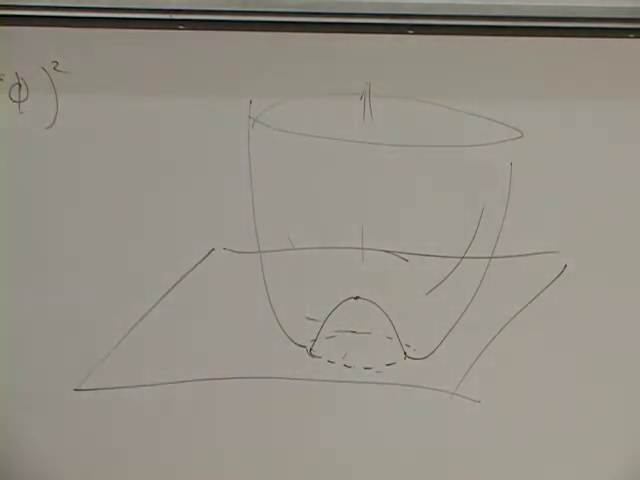
\includegraphics[width=0.72\textwidth]{lecture_07_figure_06.png}
\caption{回転面として描かれた対称性の破れたポテンシャル。原点は不安定であり、縮退した極小が円形の谷をなす。}
\lectureframe{00:37:25}
\end{figure}

場を、通常の空間の各点においてこの内部平面内の小さな矢印であると考える。ポテンシャルはすべての矢印に長さ\(f\)をもつことを要求する。勾配エネルギーは近くの矢印がほぼ同じ向きを指すことを要求する。その結果、基底状態はどこでも同じ角度をもつが、法則によって好まれる角度はない。これが連続的自発的対称性の破れである。

\section{ドメインウォールから滑らかなねじれへ}

境界の実験を繰り返す。左の境界では場を真空点\(A\)に固定し、右では別の真空点\(B\)に固定する。局在した跳びは勾配を大きくするであろう。しかし離散的な場合とは異なり、場はポテンシャルの底にとどまりながら円の周りを連続的に変化することができる。

低エネルギーでは場を\(\phi=f e^{i\alpha(x)}\)と書く。1次元空間では、関係するエネルギーは
\begin{equation}
  E[\alpha]
  =f^2\int_0^L dx\,\left(\frac{d\alpha}{dx}\right)^2.
  \label{eq:l07-angle-functional}
\end{equation}
である。端点の角度を固定すると、変分により
\begin{equation}
  \frac{d^2\alpha}{dx^2}=0,
  \qquad
  \alpha(x)=\alpha_A+
    \frac{\alpha_B-\alpha_A}{L}\,x.
  \label{eq:l07-linear-twist}
\end{equation}
が得られる。好ましい配置はねじれを試料全体に一様に広げる。そのエネルギーは
\begin{equation}
  E_{\rm twist}
  =f^2\frac{(\alpha_B-\alpha_A)^2}{L},
  \label{eq:l07-twist-energy}
\end{equation}
のようにスケールするので、\(L\)を大きくすることによりいくらでも安くすることができる。

\begin{figure}[htbp]
\centering
\begin{adjustbox}{max width=\linewidth}
\begin{tikzpicture}[x=0.95cm,y=0.95cm]
  \begin{scope}
    \draw[->] (0,0) -- (6.2,0) node[right] {$x$};
    \draw[->] (0,0) -- (0,3.5) node[above] {$\alpha(x)$};
    \draw[very thick,blue!70!black] (0.45,0.65) -- (5.7,2.85);
    \fill (0.45,0.65) circle (1.8pt) node[left] {$\alpha_A$};
    \fill (5.7,2.85) circle (1.8pt) node[right] {$\alpha_B$};
    \node at (3.1,-0.65) {physical space};
  \end{scope}
  \begin{scope}[xshift=9.2cm,yshift=1.65cm]
    \draw[thick] (0,0) circle (1.8);
    \fill (1.55,-0.92) circle (1.8pt) node[below right] {$A$};
    \fill (-0.45,1.74) circle (1.8pt) node[above] {$B$};
    \draw[very thick,blue!70!black,-{Latex[length=2.5mm]}]
      (1.55,-0.92) arc[start angle=-31,end angle=104,radius=1.8];
    \node at (0,-2.35) {vacuum circle};
  \end{scope}
\end{tikzpicture}
\end{adjustbox}
\caption{2つの記述における同じ低エネルギー配置。角度は物理空間にわたって線形に変化し、場は内部空間における真空円の短い弧に沿う。}
\end{figure}

\begin{classroomqa}
\audiencequestion{円の周りを回る方法は2通りありうる。場はどちらの経路をとるのか、またより長い方に捕らわれることがありうるか。
\lecturetimestamp{00:41:54}}
\lecturerresponse{一般的な端点に対しては、より短い角度経路の方が勾配が小さく、したがってエネルギーが低い。正反対の端点は2つの最も単純な経路を縮退させる。端点をゆっくり動かして準備された配置は余分な巻き数を保持してエネルギー障壁の背後に捕らわれることがありうるが、指定された1対の通常の端点に対しては、ねじれのない最短経路が基底状態である。}
\end{classroomqa}

\begin{classroomqa}
\audiencequestion{経路が谷の底を離れて内部を横切り、全体としてより短くなることがありうるか。\lecturetimestamp{00:43:32}}
\lecturerresponse{低エネルギーで長い試料の領域では、動径方向のポテンシャルを登るのは得にならない。半径をその真空値に保ち角度を線形に変化させることが有効エネルギーを最小化する。これは上記の変分法の計算が示すとおりである。特定のポテンシャルをもつ有限系では動径方向と角度方向の運動を同時に最小化することができるが、ゴールドストーンの結論は、谷に沿った滑らかな運動が勝つ任意に長い波長の極限に関するものである。}
\end{classroomqa}

\begin{classroomqa}
\audiencequestion{円形の谷が傾き、ある角度がより低くなったら何が変わるか。\lecturetimestamp{00:44:33}}
\lecturerresponse{その場合、対称性は明示的に破れている。1点が真の基底状態となり、円に沿った運動は復元力をもち、角度方向の励起はもはや厳密に質量ゼロではなくなる。}
\end{classroomqa}

\section{ゼロ運動量振動の代償としての質量}

滑らかなねじれは、エネルギーが勾配のみから生じる場を明らかにする。それがなぜ質量ゼロの粒子を意味するかを理解するために、相対論的分散関係
\begin{equation}
  \omega^2=\bm{k}^2+m^2.
  \label{eq:l07-dispersion}
\end{equation}
を比較する。波\(e^{i(\bm{k}\cdot\bm{x}-\omega t)}\)は運動量\(\bm{k}\)を運ぶ。
\(m=0\)ならば、そのエネルギーは波長が無限大に近づくにつれてゼロに近づく：
\(\omega=|\bm{k}|\to0\)。\(m\ne0\)ならば、空間的に一様なモード\(\bm{k}=0\)は依然として振動数\(\omega=m\)で振動する。質量は、これ以上還元できないゼロ運動量のエネルギーである。

この同じ区別はラグランジアンにも見える。項
\begin{equation}
  -\frac12m^2\varphi^2
\end{equation}
は、一様な変位に対しても復元力を与える。微分項のみをもつ場にはそのような復元力はない。その波長をより長くすれば、勾配エネルギーはゼロに近づく。

\subsection{極座標変数が2つのモードを分離する}

破れた複素場を次のように書く。
\begin{equation}
  \phi(x)=\rho(x)e^{i\alpha(x)}.
  \label{eq:l07-polar}
\end{equation}
\(\rho\) と \(\alpha\) はどちらも場である。微分すると
\begin{align}
  \partial_\mu\phi
  &=e^{i\alpha}
    \left(\partial_\mu\rho+i\rho\,\partial_\mu\alpha\right),\\
  \partial_\mu\phi^*
  &=e^{-i\alpha}
    \left(\partial_\mu\rho-i\rho\,\partial_\mu\alpha\right).
\end{align}
となり、交差項は相殺されて
\begin{equation}
  \partial_\mu\phi^*\,\partial^\mu\phi
  =(\partial_\mu\rho)(\partial^\mu\rho)
   +\rho^2(\partial_\mu\alpha)(\partial^\mu\alpha).
  \label{eq:l07-polar-kinetic}
\end{equation}
が残る。\(\phi^*\phi=\rho^2\) であるから、
\begin{equation}
  \mathcal L
  =(\partial\rho)^2+\rho^2(\partial\alpha)^2-V(\rho^2).
  \label{eq:l07-polar-lagrangian}
\end{equation}
である。ポテンシャルには \(\rho\) は含まれるが \(\alpha\) は含まれない。この不在こそが、最も有用な形での対称性である。

\begin{figure}[htbp]
\centering
\includegraphics[width=0.88\textwidth]{lecture_07_figure_03.png}
\caption{極座標場のラグランジアン、その枠囲みされた低エネルギー角度項、および対称性の破れのポテンシャル。動径方向の運動はポテンシャルを登り、角度方向の運動は谷底に沿う。}
\lectureframe{00:56:40}
\end{figure}

非常に低エネルギーの励起に対しては、場は \(\rho=f\) の近くにとどまる。すると
\begin{equation}
  \mathcal L_{\rm angular}
  \simeq f^2(\partial_\mu\alpha)(\partial^\mu\alpha).
\end{equation}
となる。\(1/2\) の因子に用いる規約を除いて、正準規格化された角度場を
\begin{equation}
  \beta=\sqrt{2}\,f\alpha,
  \qquad
  \mathcal L_{\rm angular}
  =\frac12(\partial_\mu\beta)(\partial^\mu\beta).
  \label{eq:l07-goldstone-field}
\end{equation}
によって定義する。\(\beta^2\) 項は存在しない。この角度場の量子は質量ゼロである。それらはゴールドストーンボソンである。

動径場は異なる振る舞いをする。\(\rho\) を至るところで一斉に \(f\) からずらすと、それは引き戻され、行き過ぎて、谷底のまわりを振動する。\(\rho=f+h\) ならば、式~\eqref{eq:l07-mexican-hat} の展開により
\begin{equation}
  V(f+h)=V(f)+\frac12m_h^2h^2+\cdots,
\end{equation}
が得られるので、\(h\) は質量をもつ。幾何学的には、角度方向は平坦であり、動径方向は曲がっている。

\begin{classroomqa}
\audiencequestion{場を動径方向にずらした場合、それは単に落下して戻るのか、そしてその次に何が起こるのか。\lecturetimestamp{00:57:10}}
\lecturerresponse{角度方向の運動がなければ、それは最小値に向かって落ち、行き過ぎて、動径方向に振動する。一様な振動は空間運動量がゼロであるが振動数は非ゼロであり、その振動数が動径励起の質量である。対照的に、一様な角度方向のずれは別の真空に到達し、復元力をもたない。}
\end{classroomqa}

これが、この例におけるゴールドストーン原理の内容である。連続的な大域的対称性を自発的に破ると、真空多様体の独立な平坦方向ごとに質量ゼロのモードが生じる。
\editorialnote{この主張は相対論的場の理論の通常の条件を仮定している。非相対論的多体系では、南部--ゴールドストーンモードの数え上げと分散はより微妙になり得るが、この相対論的 \(U(1)\) 模型については、講義の長波長極限の結論は依然として正しい。}

\section{スピン波、弦、および音}

この定理は抽象的であるが、その機構は身近である。等方的な強磁性体では、すべてのスピンを一緒に回転させてもエネルギーは変わらない。向きを試料全体にわたって非常にゆっくり変化させると、スピン波が得られる。そのコストは波数とともに消えるので、これは破れたスピン回転対称性のゴールドストーンモードである。

長い弾性弦は別の描像を与える。重力を無視し、弦全体を鉛直方向に並進できるように端を固定する。一様な鉛直並進はエネルギーを要しない。その並進を弦に沿ってゆっくり変化させると、長波長の横波になる。一様な対称操作が、穏やかな位置依存の変形へと昇格したのである。

\begin{figure}[htbp]
\centering
\includegraphics[width=0.68\textwidth]{lecture_07_figure_04.png}
\caption{ゴールドストーンモードの類推の際に描かれた、ゆっくり変化する弦のプロファイル。物理的な要点は、長波長変形の小さな傾きであり、曲線の鉛直方向の位置ではない。}
\lectureframe{01:04:19}
\end{figure}

\begin{classroomqa}
\audiencequestion{弦は運動量がゼロでありながら振動エネルギーを運ぶことができるのか。\lecturetimestamp{01:04:41}}
\lecturerresponse{鉛直方向の力学的運動量と、弦に沿った波の運動量とを区別しなければならない。定在波は \(+k\) と \(-k\) のモードの重ね合わせであるため正味の運動量がゼロであり得るが、それでもエネルギーを運ぶ。場の理論の類推では、運動量は軸に沿った波数を指し、鉛直変位は内部場座標を表す。}
\end{classroomqa}

スリンキーは縦波版を与える。理想化された無限に長いスリンキーをその軸に沿って全体として並進させても何も変わらない。隣り合う部分をわずかに異なる量だけ並進させると、穏やかな圧縮波が得られる。固体や流体でも、長波長の音は同様に集団的変位と密度変動から生じる。スピン波、弦の横波、および音は同じ微視的励起ではないが、決定的なパターンを共有している。一様な連続的操作はエネルギーを要せず、そのゆっくり変化する版が軟モードになるのである。
\editorialnote{結晶では、音響フォノンは慣例的に、自発的に破れた連続的並進対称性の南部--ゴールドストーンモードとして記述される。弦とスリンキーは、同じ微分のみのエネルギー構造を明らかにするために講義で用いられた力学的類推である。}

この用語は、ちょっとした教室での冗談に値するほど重要である。これらは Jeffrey Goldstone にちなんで名付けられた\emph{Goldstone}ボソンであり、ゲージボソンではない。講義は、Goldstone が Susskind の友人であったことに触れ、その後、真に異なる主題であるゲージ不変性へと移る。

\section{大域的位相対称性からゲージ対称性へ}

\(U(1)\)位相対称性は、電荷の保存に対応する対称性として、すでにこの講義に現れている。荷電粒子場は複素数であり、そのような場に共通の位相を掛けても、大域的理論は変わらない。electric という語を直観のために用いてもよいが、その電荷は別の\(U(1)\)量子数を表していてもよい。実光子は質量がなく、最終的な目標は、質量をもつ\(Z\)のような光子様の場である。

新しい問いは、\begin{equation}
  \phi'(x)=e^{i\theta(x)}\phi(x)
  \label{eq:l07-local-u1}
\end{equation}が、\(\theta\)が時空を通じて任意に変化するときに対称性であり得るか、というものである。関数\(\theta(x)\)は変換パラメータであり、追加の力学場ではない。この提案を微分によって検証する：\begin{equation}
  \partial_\mu\phi'
  =e^{i\theta}
   \left[\partial_\mu\phi+i(\partial_\mu\theta)\phi\right].
  \label{eq:l07-local-derivative}
\end{equation}。この余分な項は、\(\theta\)が定数のときには存在しなかった。共役については、\begin{equation}
  \partial_\mu\phi^{*\prime}
  =e^{-i\theta}
   \left[\partial_\mu\phi^*-i(\partial_\mu\theta)\phi^*\right].
\end{equation}。これらの積は\begin{align}
  \partial_\mu\phi^{*\prime}\partial^\mu\phi'
  ={}&
  \partial_\mu\phi^*\partial^\mu\phi
  i\left(
      \phi\,\partial_\mu\phi^*
      -\phi^*\partial_\mu\phi
    \right)\partial^\mu\theta
  \nonumber\\
  &+\phi^*\phi\,
    \partial_\mu\theta\,\partial^\mu\theta.
  \label{eq:l07-local-failure}
\end{align}である。ポテンシャルは\(\phi^*\phi\)が不変であるため不変のままだが、通常の運動項は失敗する。大域的対称性は自動的に局所的対称性になったわけではない。

\begin{classroomqa}
\audiencequestion{メキシカンハットの描像では、この失敗は円形の谷の周りに凹凸があることを意味するのですか。\lecturetimestamp{01:19:37}}
\lecturerresponse{いいえ。ポテンシャルは角度方向に完全に平坦なままであり得る。追加のコストは、位相が時空のある点から別の点へ異なるときの勾配から生じる。それは谷の起伏ではなく、通常の微分項が空間的変化を検出しているのである。}
\end{classroomqa}

\subsection{補償するベクトル場}

自然界の光子、\(W\)、\(Z\)、グルーオン相互作用は、単なる剛直な変換ではなく、局所ゲージ対称性によって組織されている。局所位相操作を対称性にするには、四元ベクトル場\(A_\mu\)によって理論を拡大する。電磁気学では\(A_0\)はスカラーポテンシャルであり、3つの空間成分がベクトルポテンシャルを形成する。それらの微分が電場と磁場を構成する。

内部的に整合する規約を選ぶ：\begin{equation}
  \phi'=e^{i\theta}\phi,
  \qquad
  A'_\mu=A_\mu-\partial_\mu\theta,
  \qquad
  D_\mu=\partial_\mu+iA_\mu.
  \label{eq:l07-gauge-convention}
\end{equation}。板書では、相殺を確認する際に1つの符号を変える。式\eqref{eq:l07-gauge-convention}が3つの符号をまとめて固定する。ゲージ結合と電荷は一時的に\(A_\mu\)に吸収されている。\editorialnote{明示的な電荷\(q\)と結合\(g\)を用いれば、\(D_\mu=\partial_\mu+igqA_\mu\)および\(A'_\mu=A_\mu-(gq)^{-1}\partial_\mu\theta\)と書ける。講義では、相殺を見やすく保つためにこれらの定数を省略している。}

共役場については、\begin{equation}
  D_\mu\phi^*=\partial_\mu\phi^*-iA_\mu\phi^*.
\end{equation}。ここで\begin{align}
  D'_\mu\phi'
  &=
  \left(\partial_\mu+iA'_\mu\right)e^{i\theta}\phi
  \nonumber\\
  &=
  e^{i\theta}
  \left[
    \partial_\mu\phi+i(\partial_\mu\theta)\phi
    +i(A_\mu-\partial_\mu\theta)\phi
  \right]
  \nonumber\\
  &=e^{i\theta}D_\mu\phi.
  \label{eq:l07-covariant-transform}
\end{align}。\(\theta\)の望ましくない微分は、\(A_\mu\)の変換によって相殺される。同様に、\begin{equation}
  D'_\mu\phi^{*\prime}=e^{-i\theta}D_\mu\phi^*.
\end{equation}。これらの積は不変である。\emph{共変}という形容詞は、微分が場自体と同じ単純な仕方で変換することを意味する。

\section{ゲージ場の力学}

\(A_\mu\)を微分を修復するためだけに導入すると、それ自身の力学をもたないままになる。ゲージ不変な場の強さは\begin{equation}
  F_{\mu\nu}
  =\partial_\mu A_\nu-\partial_\nu A_\mu.
  \label{eq:l07-field-strength}
\end{equation}である。これは反対称であるから、\(F_{\mu\mu}=0\)。その時間--空間成分は電場を含み、空間--空間成分は磁場を含む。よく知られた3ベクトル言語では、電磁エネルギー密度は\(\bm E^2+\bm B^2\)に比例するが、ローレンツ的ラグランジアンは\(\bm E^2-\bm B^2\)に比例し、符号は計量の規約に依存する。

\begin{classroomqa}
\audiencequestion{電磁場のエネルギーとラグランジアンは何ですか。\lecturetimestamp{01:33:20}}
\lecturerresponse{エネルギーは\(E^2+B^2\)から構成され、ラグランジアンは\(E^2-B^2\)を用いる。共変的には、後者は\(F_{\mu\nu}F^{\mu\nu}\)の慣用的な倍数として書かれる。反対称テンソルはベクトルポテンシャルの四次元回転である。}
\end{classroomqa}

場の強さそれ自身はゲージ不変である：\begin{align}
  F'_{\mu\nu}
  &=
  \partial_\mu(A_\nu-\partial_\nu\theta)
  -\partial_\nu(A_\mu-\partial_\mu\theta)
  \nonumber\\
  &=
  F_{\mu\nu}
  -\partial_\mu\partial_\nu\theta
  +\partial_\nu\partial_\mu\theta
  =F_{\mu\nu}.
  \label{eq:l07-field-strength-invariant}
\end{align}。最後の等式は、通常の混合偏微分が可換であることから従う。したがって標準的なゲージ不変ラグランジアンは、計量に対して選ばれた符号と規格化の規約を除いて\begin{equation}
  \boxed{
  \mathcal L
  =(D_\mu\phi)^*D^\mu\phi
  -V(\phi^*\phi)
  -\frac14F_{\mu\nu}F^{\mu\nu}}
  \label{eq:l07-scalar-qed}
\end{equation}である。

\begin{figure}[htbp]
\centering
\includegraphics[width=0.84\textwidth]{lecture_07_figure_05.png}
\caption{板書上の共変微分と組み立てられたゲージ不変ラグランジアン。変換構造が見えるように、そこでは数値因子が省略されている。}
\lectureframe{01:38:45}
\end{figure}

この構成は大域的\(U(1)\)対称性を局所的なものへ昇格させるが、それは代償---を払って、あるいは物理的には新たなベクトル場という贈り物---とともに、そうする。その場は、アーベル的例子における電磁ポテンシャルである。

\begin{classroomqa}
\audiencequestion{我々が最初に置いたラグランジアンは通常の微分を用いていた。なぜそれを共変微分に置き換え、その結果を真の理論と呼ぶことが許されるのか。\lecturetimestamp{01:42:55}}
\lecturerresponse{我々は別の、拡大された理論を構成している。すなわち、荷電物質とゲージ場である。局所ゲージ不変性がそれらの結合を決定する。得られる量子論は首尾一貫した数学的構造であり、自然が光子と弱ゲージ場をどのように組織しているかと一致する。相対論的ベクトル場を無整合に結合するだけでは、非物理的な偏極や確率の破れを導入しうるので、ゲージ原理は古い自由スカラー理論の見かけ上の書き換えではない。}
\end{classroomqa}

\begin{classroomqa}
\audiencequestion{では、新しい場を加えることがこの変更の本質的な正当化なのか。\lecturetimestamp{01:44:57}}
\lecturerresponse{はい。\(A_\mu\)がなければ、局所的に回転された場の微分には打ち消されない\(\partial_\mu\theta\)が含まれる。\(A_\mu\)とその変換則があれば、打ち消しがうまくいく。幾何学的な言葉では\(A_\mu\)は束上の接続である。そのより深い数学は実在し有用であるが、上記の代数にここで必要な部分が含まれている。}
\end{classroomqa}

\section{裸のゲージボソン質量が禁じられる理由}

通常のボソン場では、質量は二次の項で表される。次の項を加えたくなる。
\begin{equation}
  \Delta\mathcal L_{\rm Proca}
  =\frac12m^2A_\mu A^\mu.
  \label{eq:l07-proca}
\end{equation}
しかし\(A_\mu\mapsto A_\mu-\partial_\mu\theta\)の下で、
\begin{equation}
  A'_\mu A^{\mu\prime}
  =
  A_\mu A^\mu
  -2A^\mu\partial_\mu\theta
  +\partial_\mu\theta\,\partial^\mu\theta,
\end{equation}
となるので、式~\eqref{eq:l07-proca}はゲージ不変ではない。局所対称性を保ちながら、このゲージ理論に質量を手で入れることはできない。

\begin{figure}[htbp]
\centering
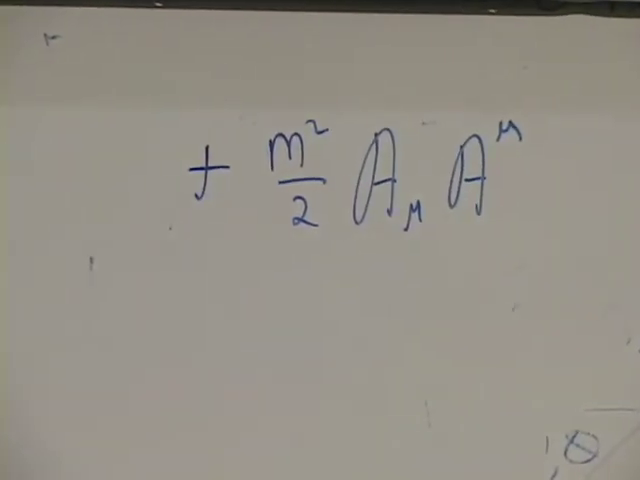
\includegraphics[width=0.72\textwidth]{lecture_07_figure_07.png}
\caption{提案された裸のベクトル質量
\(\tfrac12m^2A_\mu A^\mu\)。\(A_\mu\mapsto A_\mu-\partial_\mu\theta\)の下でのその失敗が、ヒッグス機構を準備する障害である。}
\lectureframe{01:39:48}
\end{figure}

これが見かけ上の行き詰まりである。ゲージ不変性は質量のない光子を説明し、理論を非物理的な自由度から守るが、\(W\)と\(Z\)は質量をもつ。逃げ道は明示的なベクトル質量ではありえない。それはゲージ不変なラグランジアンにすでに存在する場から生じなければならない。

\begin{classroomqa}
\audiencequestion{ゲージ不変性を導入すること自体がゴールドストンボソンを生み出すのか。\lecturetimestamp{01:45:51}}
\lecturerresponse{いいえ。ゴールドストンボソンは、ベクトルポテンシャルが導入される前に、連続な\emph{大域}対称性が自発的に破れたときに生じた。いったん対称性が局所になると、変化する位相は\(A_\mu\)によって補償されうる。破れたゲージ理論では、角度モードはもはや独立な質量のない粒子ではなく、今や質量をもつベクトル場に追加の偏極を供給する。次の講義では、その主張を単に宣言するのではなく導出する。}
\end{classroomqa}

\begin{classroomqa}
\audiencequestion{これらは川が蛇行する理由を説明するのか。\lecturetimestamp{01:47:03}}
\lecturerresponse{ここでは直接の関連は知られていない。流体の渦や生物の形でさえ、対称性の方法で記述できることは確かであり、予想外の場所に場の理論の考えを見出しても決して驚くべきではないが、この講義は川の蛇行のゲージ理論を主張するものではない。}
\end{classroomqa}

\section{講義が止まる場所}

ここで、冒頭で約束した二つの材料がそろった。真空の円をもつ連続な大域対称性には平坦な角度方向があり、そのゆっくりした変化は質量のないゴールドストン場である。局所対称性はゲージ接続と共変微分を要求し、式~\eqref{eq:l07-proca}における直接のベクトル質量を禁じる。

次の段階は、式~\eqref{eq:l07-scalar-qed}のゲージ不変理論の中で式~\eqref{eq:l07-mexican-hat}の破れたポテンシャルを用いることである。すると二つのことが同時に起こる。すなわち、別個のゴールドストン粒子は物理的スペクトルから消え、ベクトル場は質量を獲得する。通常の教育的な言葉ではゲージ対称性は自発的に破れている。より正確には、ゲージ冗長性は残りつつ、理論は質量をもつベクトル励起を伴うヒッグス相に入る。
\editorialnote{局所ゲージ対称性は、異なる観測可能な状態の間に作用する通常の物理的対称性ではなく、記述の冗長性である。この講義では自発的ゲージ対称性の破れという標準的な略記を用いる。ゲージ不変な物理的記述は、ヒッグス相における自由度の再編成である。}

これがヒッグス現象である。我々はまだそれを実行していない。この講義は、解が来たときに避けられないものとなるよう、問題を十分に精密にするという必要なより困難な仕事を果たした。
